\chapter{Security and Data Protection}
\label{chap:ch5}

\par Security was treated as a primary design constraint throughout the development of QuickShift, not as a feature to be retrofitted after the core functionality was complete. The application implements stateless authentication, strict role-based access control, per-store data isolation, and a secure account lifecycle that covers both self-service password management and administrator-led provisioning of privileged accounts. This chapter describes each of these mechanisms in detail, explaining both the technical implementation and the threat model each control addresses.

%-----------------------------------------------------------
\section{Authentication Architecture and JWT-Based Sessions}
%-----------------------------------------------------------
\par The backend uses JSON Web Tokens (JWTs) as the sole session mechanism. When a user authenticates via the \texttt{/api/auth/login} endpoint, the server validates the provided credentials against the stored hashed password and, if successful, generates a signed JWT containing the user's identifier (as the subject, represented by the user's email address). The token is returned to the client and must be included as a Bearer token in the \texttt{Authorization} header of every subsequent request. \cite{JWTDepth}

\par Token validation is performed by a \texttt{JwtAuthenticationFilter} that intercepts requests before they reach any controller. The filter extracts the token from the \texttt{Authorization} header, verifies its signature and expiration using the server-side secret key, and then loads the user details via the configured \texttt{UserDetailsService}. This step queries the database on each authenticated request to obtain the current user and authorities. The filter populates Spring Security's \texttt{SecurityContext} with a \texttt{UsernamePasswordAuthenticationToken}, so controllers and service methods can access the current user through the standard \texttt{Authentication} object.

\par The stateless model eliminates server-side session storage and the associated concurrency and scalability concerns. It also mitigates the possibility of session fixation attacks, since there is no server-maintained session that an attacker could hijack by obtaining a pre-authentication identifier. The trade-off is that token revocation requires either short expiry windows or a token blacklist; the current implementation uses a fixed expiry duration configured via application properties, which is appropriate for the expected usage patterns of a store management tool.\cite{Stateless}

\par Because the token only carries the subject (user email) and not roles, authorization decisions rely on the authorities loaded from the database during the filter phase. This is much safer, because any role change or account disablement takes effect immediately, even if a previously issued token is still valid. Those authorities are then available for downstream access checks through Spring Security.

\begin{figure}[H]
    \centering
    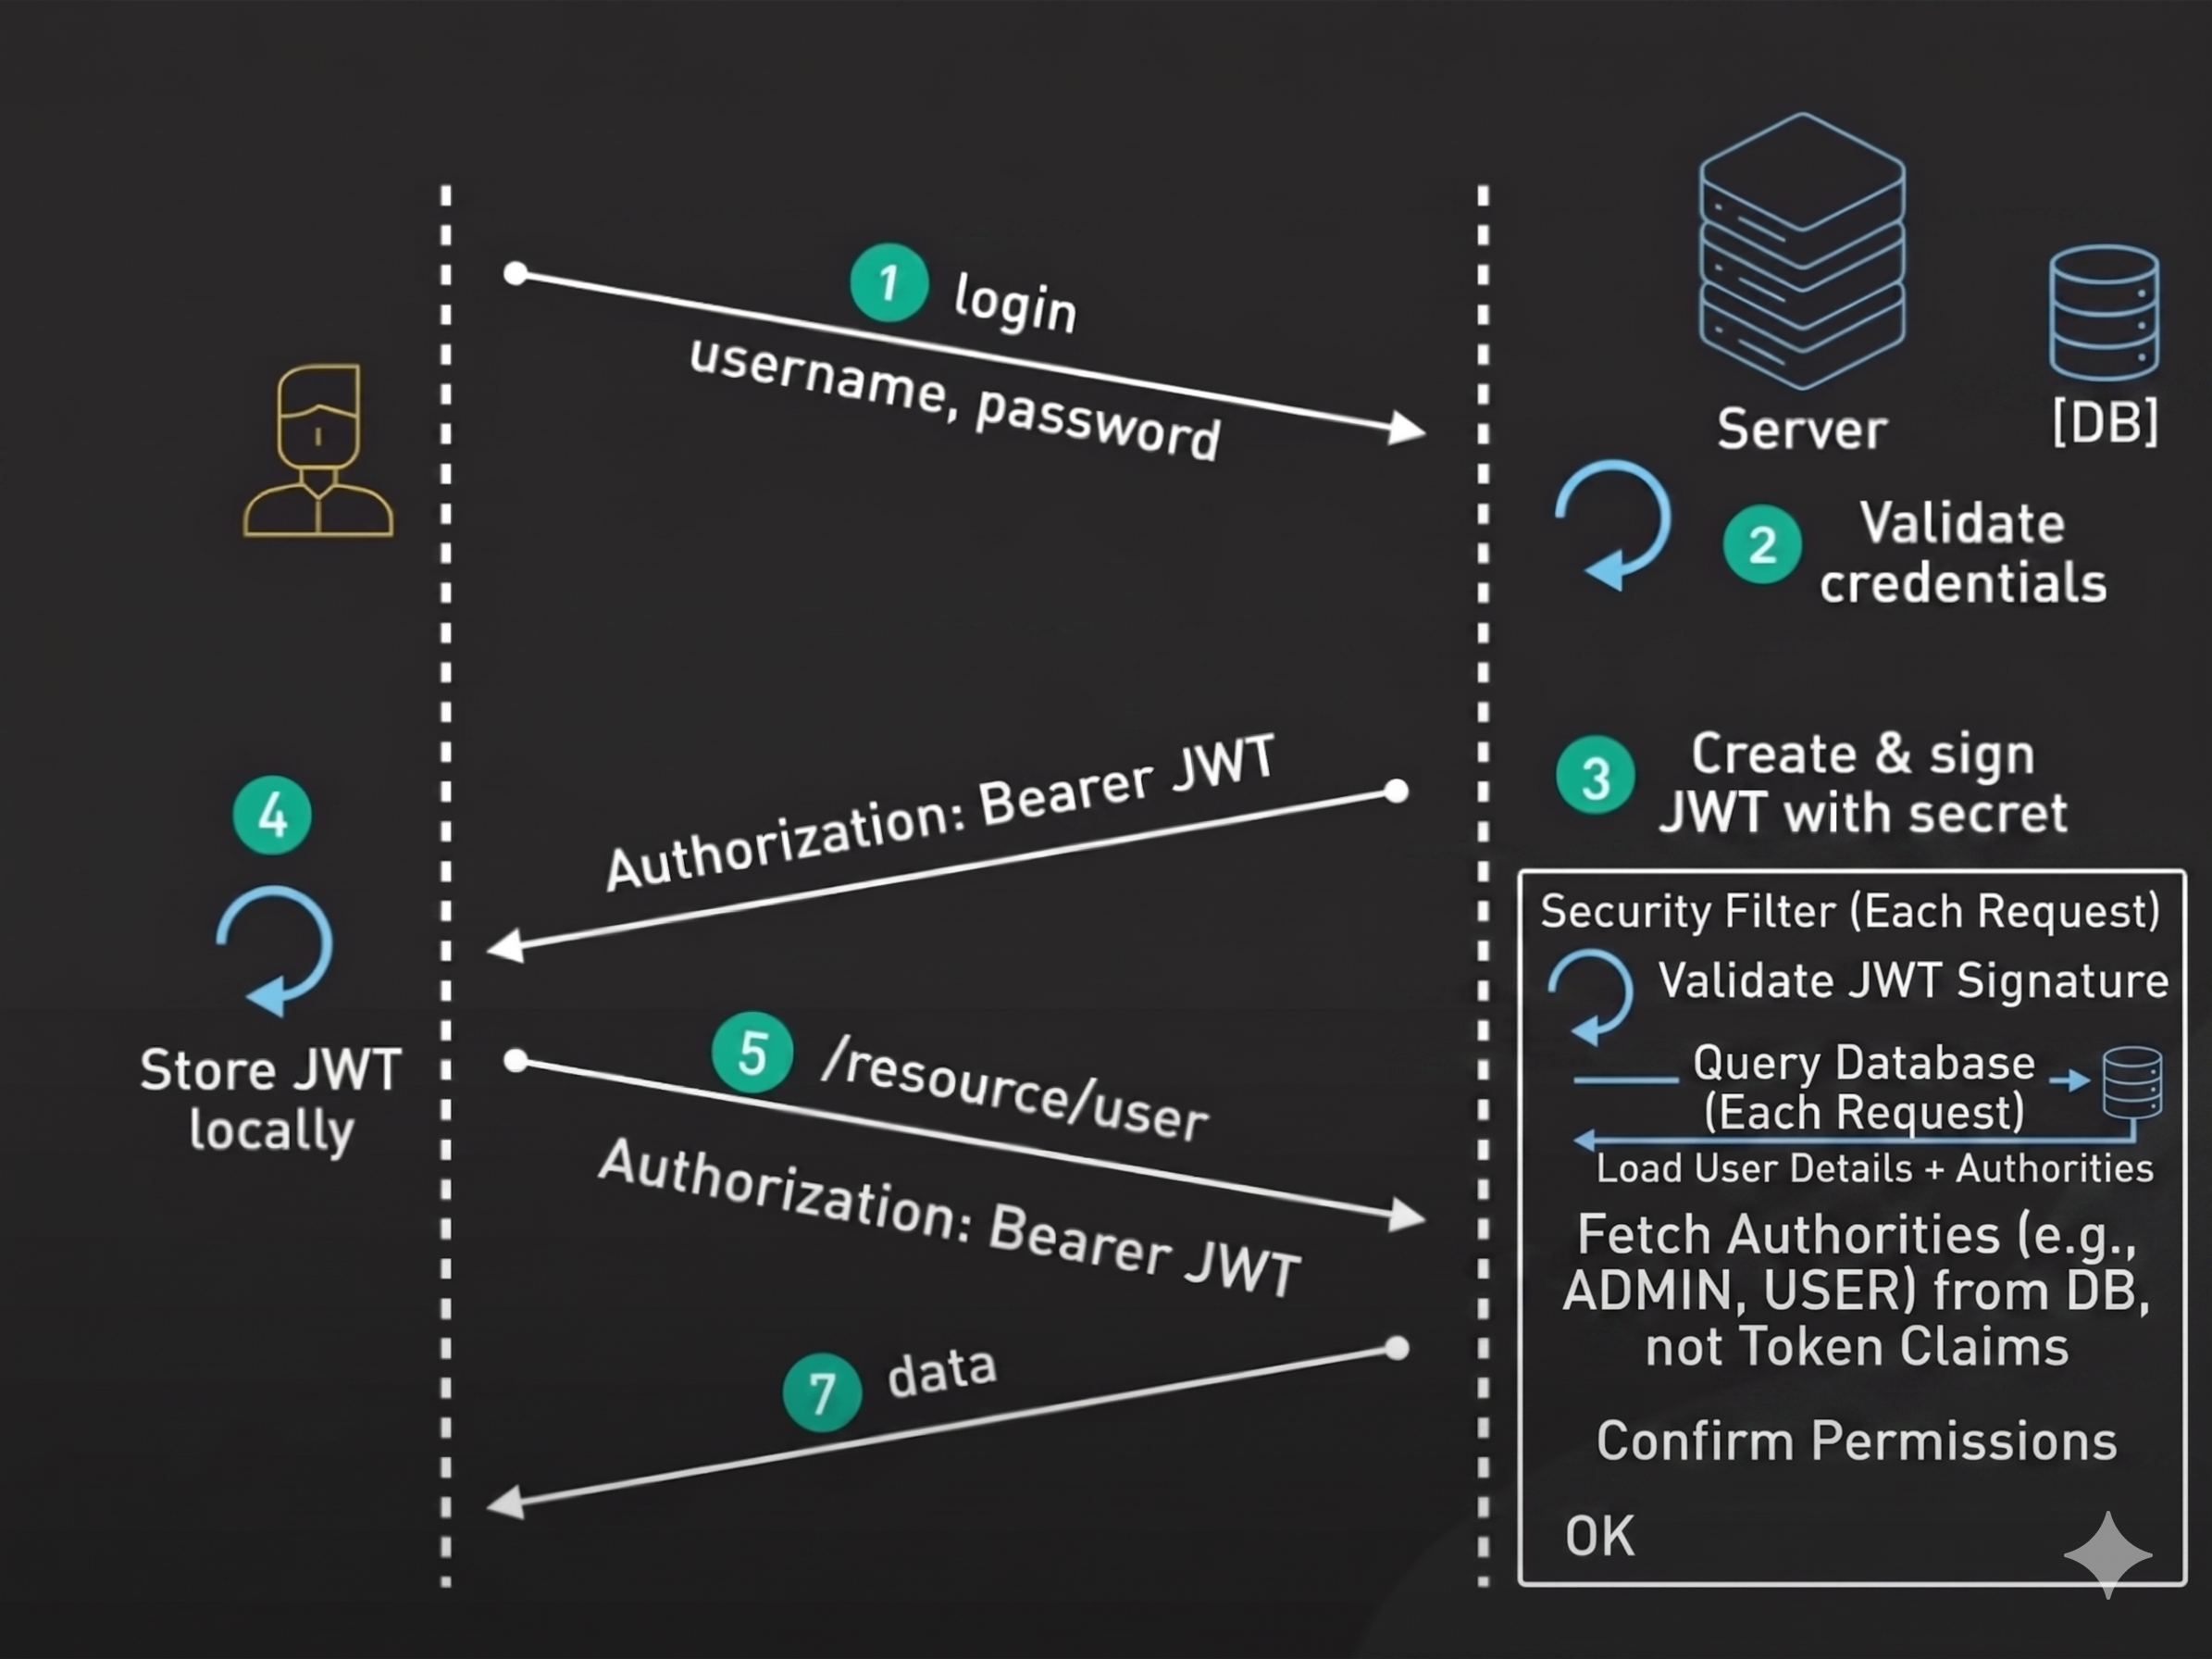
\includegraphics[width=1\linewidth]{Stateless.png}
    \caption{Stateless Authentication Visual}
    \label{fig:placeholder}
\end{figure}

%-----------------------------------------------------------
\section{Role-Based Access Control}
%-----------------------------------------------------------
\par The system defines three roles: \texttt{EMPLOYEE}, \texttt{MANAGER}, and \texttt{ADMIN}. Access control is enforced at two levels: at the HTTP layer through Spring Security's URL-based rules, and at the controller method level through explicit role checks.\cite{RBAC1}

\par URL-based rules in \texttt{SecurityConfig} restrict access to sensitive endpoint prefixes by role. For example, administrative endpoints such as store creation and manager provisioning are restricted to the \texttt{ADMIN} role, while schedule generation and absence acknowledgment are restricted to \texttt{MANAGER} and \texttt{ADMIN}. The remaining employee-facing endpoints are accessible to all authenticated users, with finer-grained ownership checks performed inside the service layer.


\par Method-level checks complement the URL rules for cases where the same endpoint serves multiple roles but must return or accept different data depending on who is calling. For example, the shift listing endpoint returns all shifts for a store when called by a manager, but only personal shifts when called by an employee. This branching logic is implemented in the controller by inspecting the role from the \texttt{Authentication} object and delegating to the appropriate service method.

\par The role separation also limits the blast radius of a compromised credential. An employee account cannot be used to access the schedule generation endpoint, acknowledge absences, or view another employee's personal data. A manager account cannot access global administrative operations such as creating new stores or provisioning other managers. This defense-in-depth approach ensures that even if an account is compromised, the attacker's capabilities are confined to the role's intended scope. \cite{RBAC2}

\begin{center}
\begin{tabular}{c}
Authentication Filter \\
$\downarrow$ \\
JWT Validation \\
$\downarrow$ \\
User Lookup \\
$\downarrow$ \\
Authority/Role Lookup \\
$\downarrow$ \\
Permission Evaluation \\
$\downarrow$ \\
Controller/Resource \\
\end{tabular}
\end{center}

%-----------------------------------------------------------
\section{Store-Scoped Data Isolation}
%-----------------------------------------------------------
\par QuickShift is designed as a multi-tenant system in which each store operates as an isolated organizational unit. Data isolation is enforced at the query level: every repository method that returns operational data (shifts, employees, leave requests, absence requests) accepts a store identifier as a parameter and filters results accordingly.

\par When a manager makes a request, their associated store identifier is extracted from their \texttt{AppUser} entity (which is loaded during the authentication filter phase) and injected into the query. This happens transparently at the service layer, so managers cannot access or modify data from stores they do not own simply by supplying a different store ID in the request body. The service method resolves the store from the authenticated user's identity rather than trusting the client-supplied value.

\par Administrators occupy a special position in this model: they are not assigned to a specific store and can therefore pass explicit store identifiers in requests. Administrative endpoints validate that the supplied store ID corresponds to an existing store before proceeding, so even administrators cannot target non-existent stores. Global operations (such as listing all employees across all stores) are available only to administrators and not to managers.

\par This isolation model prevents horizontal privilege escalation between tenants: a compromised manager account for store A cannot be used to read or modify data for store B, since the store association is enforced server-side from the authenticated identity rather than from any client-controlled parameter.

\begin{figure}[H]
\centering
\begin{tikzpicture}[
    node distance=4cm and 4cm, % Increased vertical distance to prevent overlapping
    role/.style={
        rectangle,
        rounded corners,
        draw=black,
        thick,
        minimum width=4cm,
        minimum height=1.2cm,
        align=center,
        fill=gray!10
    },
    access/.style={
        rectangle,
        draw=black,
        minimum width=5.5cm, % Slightly widened to better fit the new text
        minimum height=2.2cm,
        align=left,
        fill=blue!5
    },
    arrow/.style={
        ->,
        thick
    }
]

% Roles
\node[role] (admin) {\textbf{ADMIN}};
\node[role, below=of admin] (manager) {\textbf{MANAGER}};
\node[role, below=of manager] (employee) {\textbf{EMPLOYEE}};

% Permissions
\node[access, right=4cm of admin] (adminacc) {
\textbf{Access Scope:} \\
$\bullet$ All stores \\
$\bullet$ User provisioning \\
$\bullet$ Store management \\
$\bullet$ Shift management \\
$\bullet$ Employee management \\
$\bullet$ Full administrative operations
};

\node[access, right=2cm of manager] (manageracc) {
\textbf{Access Scope:} \\
$\bullet$ Own store only \\
$\bullet$ Employee management \\
$\bullet$ Shift generation and updates \\
$\bullet$ Manual shift management \\
$\bullet$ Absence acknowledgment and replacement \\
$\bullet$ Leave request approval/disapproval \\
};

\node[access, right=4cm of employee] (employeeacc) {
\textbf{Access Scope:} \\
$\bullet$ Own store only \\
$\bullet$ View personal schedule \\
$\bullet$ Report absences \\
$\bullet$ Request Leave \\
};

% Arrows
\draw[arrow] (admin) -- (adminacc);
\draw[arrow] (manager) -- (manageracc);
\draw[arrow] (employee) -- (employeeacc);

\end{tikzpicture}

\caption{Role-based access control hierarchy and permission scope.}
\label{fig:rbac}
\end{figure}

%-----------------------------------------------------------
\section{Secure Password Management and Recovery}
%-----------------------------------------------------------
\par To protect user credentials throughout their lifecycle, QuickShift implements a secure password storage strategy, an authenticated change workflow, and a time-limited recovery mechanism.

%-----------------------------------------------------------
\subsection{Password Storage and Authenticated Change Workflow}
%-----------------------------------------------------------
\par User passwords are stored exclusively in encoded form. The \texttt{PasswordEncoder} bean configured in the Spring Security context applies a strong hashing algorithm (BCrypt\cite{bcrypt1999} by default in the Spring Security ecosystem) before any password is persisted. The raw password is never stored, logged, or returned in any API response.

\par Authenticated users can change their own password through a dedicated endpoint that requires the caller to supply their current password. The endpoint verifies the current password against the stored hash before accepting the new one. This requirement prevents an attacker who has gained temporary access to an authenticated session (for example, through a shared or unattended device) from silently changing the account password and locking out the legitimate owner.

\par New passwords are immediately encoded and stored, replacing the previous hash. The old password becomes invalid at the moment the change is committed, so subsequent requests using a JWT that was issued before the change will still be valid until the token expires, since the token is not invalidated by a password change. 

%-----------------------------------------------------------
\subsection{Forgot-Password and Time-Limited Recovery Tokens}
%-----------------------------------------------------------
\par The password recovery flow is designed to be both secure and frictionless for legitimate users. When an employee or manager requests a password reset, the system generates a cryptographically random token, associates it with the requesting account, and stores it in the \texttt{PasswordResetToken} table with a 15-minute expiry and a \texttt{used} boolean flag initialized to \texttt{false}. A reset link embedding the token is then sent to the user's registered email address.

\par When the user follows the link and submits a new password, the backend validates the token in three steps as summarized in Table~\ref{tab:token_validation}.

\begin{table}[H]
\centering
\begin{tabular}{|p{3.5cm}|p{6.5cm}|p{4.5cm}|}
\hline
\textbf{Validation Check} & \textbf{Mechanism/Database Field} & \textbf{Failure Consequence} \\ \hline
Token Existence & Query by token string & Immediate rejection (Unknown Token) \\ \hline
Expiration Check & Compare \texttt{expiresAt} with current time & Rejection (Expired Token) \\ \hline
Usage Status & Verify \texttt{used} boolean flag is \texttt{false} & Rejection (Already Used Token) \\ \hline
\end{tabular}
\caption{Step-by-step token validation checks for password recovery.}
\label{tab:token_validation}
\end{table}

\par If all three checks pass, the new password is encoded and stored, and the token's \texttt{used} flag is set to \texttt{true}. This invalidates the token for any future use, preventing replay attacks in which an attacker who intercepts a reset link could apply it a second time after the legitimate user has already completed the reset.

\par The 15-minute expiry window is short enough to limit the risk of interception but long enough to accommodate realistic email delivery delays and user response times.

%-----------------------------------------------------------
\section{Input Validation and Structured Error Handling}
%-----------------------------------------------------------
\par All publicly exposed endpoints apply input validation before invoking service logic. Mandatory fields are checked for presence, date ranges are validated for logical consistency (end date must not precede start date), and string values that must match an enumerated set are validated against that set. Malformed or logically inconsistent requests are rejected with HTTP 400 and a descriptive error message before any database operation is attempted.

\par Error messages are kept concrete enough to be actionable for legitimate users but deliberately do not expose internal implementation details such as stack traces, database column names, or query structures. For 401 and 403 responses, the messages are intentionally generic to avoid leaking information about which accounts or resources exist.

\par In the frontend, error responses from the backend are displayed inline within the relevant form or notification component rather than through modal dialogs or global alert banners. This keeps the error context local to the action that caused it and reduces user confusion. Errors are cleared when the user modifies the input or retakes the relevant action.

%-----------------------------------------------------------
\section{Transactional Safeguards for Multi-Step Operations}
%-----------------------------------------------------------
\par Several operational flows in QuickShift involve multiple related writes that must either all succeed or all fail together. Table~\ref{tab:transactional_safeguards} details these critical flows and the potential inconsistencies that would arise from partial failures.

\begin{table}[H]
\centering
\begin{tabular}{|p{4.5cm}|p{9.5cm}|}
\hline
\textbf{Operational Flow} & \textbf{Atomic Actions and Inconsistency Risks} \\ \hline
\textbf{Leave Approval} & Deducting leave days, updating request status, and marking shifts as absent. A partial failure would leave the leave balance inconsistent. \\ \hline
\textbf{Replacement Offer} & Creating the replacement shift, updating the absence request status, and updating the offer status. A failure would leave the slot marked unfilled. \\ \hline
\textbf{Schedule Regeneration} & Deleting existing shifts, absence requests, and replacement offers, followed by generating the new schedule. A failure would leave the store with no schedule. \\ \hline
\end{tabular}
\caption{Critical transactional bounds and inconsistency risks.}
\label{tab:transactional_safeguards}
\end{table}

\par All service methods that perform multi-step writes use the \texttt{@Transactional} annotation  \cite{spring_transactional}, delegating the consistency guarantee to the Spring transaction manager and the underlying database. If any step in the method throws an exception, the entire transaction is rolled back and the database is restored to its state before the method was invoked.

%-----------------------------------------------------------
\section{Email Infrastructure and Security Notifications}
%-----------------------------------------------------------
\par QuickShift integrates email delivery to support both manager onboarding workflows and automated security notifications for user password resets.

%-----------------------------------------------------------
\subsection{Manager Onboarding and Account Provisioning}
%-----------------------------------------------------------
\par Manager accounts are created exclusively by administrators through a dedicated provisioning endpoint. This design prevents self-registration of privileged accounts and maintains a controlled, auditable onboarding process for store managers.

\par When an administrator provisions a new manager, the system follows the sequence of steps detailed in Table~\ref{tab:manager_provisioning}.

\begin{table}[H]
\centering
\begin{tabular}{|c|l|p{9.5cm}|}
\hline
\textbf{Step} & \textbf{Action} & \textbf{Implementation Details} \\ \hline
1 & Password Generation & Generates a secure, cryptographically random temporary password. \\ \hline
2 & User Record Creation & Creates the \texttt{AppUser} record with the \texttt{MANAGER} role and the encoded temporary password. \\ \hline
3 & Email Dispatch & Sends an onboarding email to the manager containing the credentials and setup instructions. \\ \hline
\end{tabular}
\caption{Manager account provisioning workflow sequence.}
\label{tab:manager_provisioning}
\end{table}

\par The administrator also assigns the new manager to a specific store at provisioning time, using a dropdown populated from the list of stores that do not yet have an assigned manager. This prevents creating orphaned manager accounts and keeps the store-manager relationship consistent from the moment of account creation.

%-----------------------------------------------------------
\subsection{Email Delivery for Security-Critical Communications}
%-----------------------------------------------------------
\par The application integrates with an SMTP server \cite{smtp_rfc5321} via Spring's \texttt{JavaMailSender} to deliver security-critical emails. The two primary categories of dispatched emails are summarized in Table~\ref{tab:email_categories}.

\begin{table}[H]
\centering
\begin{tabular}{|p{4.5cm}|p{9.5cm}|}
\hline
\textbf{Email Category} & \textbf{Contents and Security Scope} \\ \hline
\textbf{Password Reset Links} & Contains the reset URL with the embedded token, instructions, and a notice that the link expires in 15 minutes to prompt quick action. \\ \hline
\textbf{Manager Onboarding} & Contains the temporary password and instructions to log in and change it immediately before performing any operations. \\ \hline
\end{tabular}
\caption{Categories of security-critical email communications.}
\label{tab:email_categories}
\end{table}

\par Email delivery failures are not silently swallowed. If the mail server is unreachable or the message cannot be sent, the exception propagates to the controller, which returns an appropriate error to the calling client. This ensures that administrators are aware of delivery failures rather than believing a provisioning action succeeded when the manager never received their credentials.

%-----------------------------------------------------------
\section{Summary of the Security Architecture}
%-----------------------------------------------------------
\par The QuickShift security model is built on four independent layers that collectively provide defense in depth, as outlined in Table~\ref{tab:security_layers}.

\begin{table}[H]
\centering
\begin{tabular}{|l|p{10.5cm}|}
\hline
\textbf{Security Layer} & \textbf{Key Mechanism and Security Value} \\ \hline
\textbf{Authentication} & Stateless JWT-based sessions prevent session-related attacks and scale horizontally. \\ \hline
\textbf{Authorization} & Role-based access control at URL/method level and ownership checks in service logic. \\ \hline
\textbf{Data Isolation} & Store-scoped queries enforced server-side prevent horizontal cross-tenant access. \\ \hline
\textbf{Account Lifecycle} & BCrypt hashing, time-limited recovery tokens, and transactional email dispatch. \\ \hline
\end{tabular}
\caption{Defense-in-depth security layers in QuickShift.}
\label{tab:security_layers}
\end{table}

\par This layered design means that a weakness in one layer does not immediately compromise the entire system. An attacker who obtains a valid JWT is still constrained by role and store scope; one who gains access to the database sees only hashed passwords; one who intercepts a reset email has at most 15 minutes to use the token and cannot reuse it after the legitimate user resets their password.